\begin{apendicesenv}
\chapter{Especificação de Regras da Empresa}

\begin{description}
\item [Rotatividade de funcionários] Dentro do contexto da empresa júnior Engrena, existe a política de rotatividade adotado, se espelhando em várias outras empresas que obtiveram sucesso não apenas na satisfação do empregado, retirando o sentimento de monotonia e identificando quais características emergem do funcionário, podendo assim encaminhar o mesmo para uma área mais adequada.

\item [Desempenho dos funcionários] A Engrena possui uma grande dificuldade em identificar e exibir para os diretores como um funcionário está desempenhando o seu papel dentro da empresa, atualmente processando-se através de planilhas no Excel®, desta forma exibindo apenas resultados binários da execução de tarefas.

\item [Identificação de prováveis diretores] Dentro da política da Engrena, existe uma filosofia de promoção de funcionários através de suas habilidades e desempenho. Com o atual cenário de muitos diretores terem se formado, surgiu uma grande demanda para os cargos de diretores, porém com a vigente estrutura de reconhecimento do desempenho, esta filosofia está quase que impossibilitada.

\item [Entrada de pessoas sem experiência técnica] Por se tratar de uma empresa júnior, o ingresso de pessoas na Engrena é feito sem a necessidade obrigatória de muita experiência técnica. Isso é, o único requisito para se tornar um funcionário da empresa é estar disposto a aprender novas coisas frequentemente.

\end{description}




























\chapter{Documento de Visão}

\section{Introdução}

Este artefato tem por objetivo, descrever, para um melhor entendimento de ambas as partes
sobre as necessidades e recursos de nível superior do Engerir . Ele concentra-se nos recursos necessários aos envolvidos e ao público-alvo, além das razões que levam a essas necessidades. Os detalhes de como o EnGerir satisfaz essas necessidades são descritos no caso de uso e nas especificações suplementares.

\section{Posicionamento}
\subsection{Oportunidades de Negócios}

Dentro da disciplina de Engenharia de Requisitos, tivemos a oportunidade de estudar as necessidades da empresa júnior Engrena, a qual era controlar os seus funcionários de uma maneira mais eficiente.
Observou-se também, com base em todos os estudos prévios dentro da disciplina, a necessidade de utilizar das várias técnicas e métodos previstos na metodologia tradicional, para a resolução do problema da Engrena.


\subsection{Descrição do Problema}


\begin{table}[!h]
\centering
\caption{Problemas}
\label{problem}
\begin{tabular}{|p{7cm}|p{7cm}|}
\hline
ID                    & PB 1                                                                                                                  \\ \hline
O problema de         & gerenciar os membros e as atividades dos mesmos                                                                       \\ \hline
afeta                 & os gestores da Engrena                                                                                                \\ \hline
cujo impacto é        & diminuição na transparência das atividades dos membros, além de diminuição da rastreabilidade das entregas acadêmicas \\ \hline
uma boa solução seria & uma ferramenta de gerência completa que permita gerenciar membros e entregas acadêmicas                               \\ \hline
\end{tabular}
\end{table}

\pagebreak
\clearpage
\newpage

\subsection{Sentença de Posição do Produto}

\begin{table}[!h]
\centering
\caption{Sentença do Produto}
\label{product}
\begin{tabular}{|p{7cm}|p{7cm}|}
\hline
Para            & gestores das Engrena                                                                                                         \\ \hline
Que             & necessitam de um melhor gerenciamento na distribuição das atividades de seus membros bem como na obtenção de seus resultados \\ \hline
O               & EnGerir                                                                                                                      \\ \hline
Que             & auxilia no gerenciamento das atividades dos membros da empresa júnior                                                        \\ \hline
Ao contrário de & um software de planilha(como o MS Excel)                                                               \\ \hline
Nosso produto   & irá facilitar o gerenciamento de atividades entre os membros, bem como analisar seus desempenhos                             \\ \hline
\end{tabular}
\end{table}

\section{Descrição dos Envolvidos e dos Usuários}

Nesta seção do documento, pretende-se apresentar os envolvidos e os usuários que farão a interação com a solução aqui descrita. Além disso, haverá uma apresentação geral sobre os papéis de cada envolvido, bem como uma descrição do mesmo.
Dessa forma, pretende-se estabelecer de forma clara quem é o beneficiado da aplicação, além de todos os envolvidos que não serão usuários diretos do sistema, mas que serão afetados pelo mesmo.

\subsection{Resumo dos Envolvidos}

\begin{table}[!h]
\centering
\caption{Envolvidos do projeto}
\label{stake}
\begin{tabular}{{|p{4cm}|p{4cm}|p{4cm}|}}
\hline
Nome                                 & Descrição                                                                              & Responsabilidades                                                                               \\ \hline
Equipe de Desenvolvimento            & Estudantes da Universidade de Brasília, da disciplina de Requisitos de Software        & Desenvolver o processo e aplicá-lo com o cliente estabelecido pela disciplina                   \\ \hline
Gustavo Sabino                       & Estudante da Universidade de Brasília, monitor da disciplina de Requisitos de Software & Auxiliar a equipe de desenvolvimento na tarefa de desenvolver e aplicar o processo              \\ \hline
Professora Elaine Venson             & Professora que ministra a disciplina de Requisitos de Software                         & Auxiliar a equipe de desenvolvimento e orientar sobre a implementação                           \\ \hline
Romenigue Igor Melo Araujo Fernandes & Representante da Engrena responsável por interagir com a equipe de desenvolvimento     & Descrever a empresa e o problema, sendo fonte de requisitos para o desenvolvimento da aplicação \\ \hline
\end{tabular}
\end{table}

\newpage

\subsection{Resumo dos Usuários}

\begin{table}[!h]
\centering
\caption{Usuários do projeto}
\label{users}
\begin{tabular}{|p{4cm}|p{4cm}|p{4cm}|}
\hline
Nome                            & Descrição                                                                                          & Responsabilidades                                                                                                                                             \\ \hline
Diretores e Gestores da Engrena & Líderes de direções da empresa, responsáveis por supervisionar o andamento da empresa como um todo & No sistema, os diretores serão capazes de acompanhar o desempenho de áreas e usuários individuais. Além disso, poderão criar atividades para outros usuários. \\ \hline
Funcionários da Engrena         & Funcionários gerais da empresa, responsáveis por desempenhar funções estabelecidas pelos diretores & Verificar a existência de atividades atribuídas a si para ser capaz de fazê-las.                                                                              \\ \hline
\end{tabular}
\end{table}

\subsection{Ambiente do Usuário}

O \textit{software} será implementado via \textit{web}, sendo portanto possível a utilização pelos navegadores mais difundidos, entre eles:

\begin{itemize}
\item Google Chrome
\item Internet Explorer 9 ou superior
\item Microsoft Edge
\item Mozilla Firefox
\item Safari
\item Outros
\end{itemize}

\subsection{Principais Necessidades dos Usuários ou dos Envolvidos}

\begin{table}[!h]
\centering
\caption{Necessidades}
\label{needs}
\begin{tabular}{|p{1cm}|p{3cm}|p{2cm}|p{3cm}|p{2cm}|p{3cm}|}
\hline
ID    & Necessidade                                                                                                                & Prioridade & Preocupações                                                                & Solução Atual   & Soluções Propostas                                                                                                           \\ \hline
NE1.1 & Verificar desempenho de áreas e usuários individuais dentro da empresa. Também consultar tal informação relativo ao tempo. & Alta       & Perda de produtividade nas atividades executadas pela empresa               & Planilhas Excel & Agregação das informações relativas à entregas de atividades em forma de gráficos                                            \\ \hline
NE1.2 & Criar tarefas em um ambiente virtual compartilhado e assinalar funcionários para sua execução, com atributos               & Alta       & Falta de uma maneira de criar tarefas e rastreá-las de forma efetiva depois & Planilhas Excel & Um mecanismo capaz de criar tarefas e atribuir para determinados usuários, com os devidos atributos relativos à tais tarefas \\ \hline
\end{tabular}
\end{table}

\pagebreak
\clearpage
\newpage

\subsection{Características}

\begin{table}[!h]
\centering
\caption{Características encontradas}
\label{looks}
\begin{tabular}{|p{4cm}|p{4cm}|}
\hline
ID       & Características                            \\ \hline
CA 1.1.1 & Agregar informações                        \\ \hline
CA 1.1.2 & Mostrar desempenho de membros graficamente \\ \hline
CA 1.2.1 & Criar tarefas em um ambiente virtual       \\ \hline
CA 1.2.2 & Verificar tarefas completadas              \\ \hline
CA 1.2.3 & Criar áreas para alocamento de membros     \\ \hline
\end{tabular}
\end{table}

\subsection{Alternativas e Concorrência}

\begin{description}

\item [Moodle] Ferramenta amplamente utilizada na Universidade de Brasília. Permite o envio de atividades e atribuição de nota às mesmas, que é um dos desejos do cliente. Porém, não há a função de visualização de desempenho por gráfico.

\item [Microsoft Excel] Forma atual de gerenciamento de desempenho e de atividades da empresa. Não é muito eficiente, porém é uma alternativa barata e que os diretores já tem certa experiência.

\item [Trello] Ferramenta para gerenciamento de projetos. Forte concorrente por ser bem discriminado entre os estudantes e no mercado, o Trello é uma excelente ferramenta para gerenciamento, todavia ela não possui uma feature para gerar gráficos, o que é uma necessidade fundamental para o nosso cliente.

\end{description}

\section{Visão Geral do Produto}

\subsection{Perspectiva do Produto}

O sistema deverá auxiliar no aumento da produtividade da empresa júnior por meio de um sistema de gerenciamento de pessoas eficiente e descomplicado. O desempenho das direções e dos funcionários da empresa poderão ser vistos em gráficos que representarão a quantidade de tarefas que tal direção ou funcionário fez de todas que tinha para fazer.
Além disso, outras possibilidades estão inclusas na solução proposta, como a criação e atribuição de tarefas por parte dos diretores aos funcionários da empresa, podendo inclusive atribuir notas à essas tarefas. Por parte dos funcionários, os mesmos poderão visualizar quais tarefas foram designadas à eles, permitindo um maior planejamento e evitando situações de esquecimento de atividades.

\subsection{Suposições e Dependências}

Por se tratar de um sistema web, algumas dependências devem ser atingidas para que o mesmo funcione corretamente:

\begin{itemize}
\item Dispositivo eletrônico com \textit{software} de \textit{browser};
\item Disponibilidade de servidores;
\item Acesso à \textit{internet}.
\end{itemize}

\section{Recursos do Produto}

\begin{itemize}
\item Capacidade de gerenciar tarefas
\item Capacidade de alocar tarefas para usuários
\item Capacidade de fornecer relatórios e estatísticas sobre o desempenho de um membro
\item Capacidade de assinalar uma tarefa como terminada
\item Capacidade de gerenciar as pessoas que entram e saem da empresa
\item Capacidade de armazenar os dados dos membros
\item Capacidade de gerenciar as contas de acesso ao sistema, de forma que elas tenham diferentes níveis de acesso a este
\end{itemize}

\section{Outros Requisitos do Produto}

Será uma aplicação web, que deverá estar disponível 24 horas por dia, durante todos os dias da semana.
Ela não precisará ter um alto desempenho, como por exemplo, abrir a página em menos de 2 segundos.





















% Relato sobre o produto

\chapter{Relato sobre o Produto}


\section{Introdução}

Este documento introdutório da segunda fase do planejamento tem como objetivo apresentar de forma mais objetiva e reduzida sobre o propósito do sistema. Os problemas não serão aqui notificados, sendo uma coletânea reduzida apenas do que o sistema deve proporcionar.

\section{Sobre o Produto}

Da mesma forma como engenheiros de software precisam de ferramentas para rastrear diversos tipos de informações, uma empresa deve conseguir aferir a produtividade de seus membros e de áreas de dentro da empresa.
Tais informações podem auxiliar o aumento no desenvolvimento da corporação, visto que é um indicador de onde podem ser necessárias reestruturações e melhorias diversas.
Dessa forma, o que é objetivado é uma ferramenta de rastreamento de atividades de membros e áreas, de forma a averiguar a produtividade e qualidade das atividades produzidas pela empresa em determinados períodos de tempo.
Por ter a função supracitada, a ferramenta também permite que os gestores da empresa podem verificar a todo momento quantos membros há na empresa. Em novos processos seletivos, membros poderão ser facilmente adicionados e em processos de demissão, membros poderão ser retirados.
Além disso, a ferramenta deve ter a função de produtividade, não apenas de rastreamento. Isso significa que membros terão sua área dentro da aplicação, que os permitirá adicionar informações sobre si, como competências e capacitações. Essas informações serão utilizadas pelos gestores na alocação de pessoal a projetos específicos.
Complementando, para atingir o objetivo de produtividade, os membros também poderão visualizar tarefas criadas que foram atribuídas a si, com a data de término. Dessa forma, os mesmos poderão ter um centro de convergência de atividades para não haver atrasos nas entregas por razões de esquecimento.
Por fim, os diretores receberão uma notificação quando os membros marcarem uma atividade como feita. Então, poderão recebê-la pessoalmente e a avaliar, adicionando mais um parâmetro no quesito de rastreabilidade, isso é, qualidade e quantidade.






























% Plano de Gerenciamento de Requisitos
\chapter{Plano de Gerenciamento de Requisitos}
\label{plano_de_gerenciamento_de_requisitos}

\section{Introdução}

A finalidade deste documento é documentar como será a rastreabilidade dos requisitos, bem como quais atributos serão utilizados para classificar os mesmos. Desta forma os requisitos estarão sendo analisados, documentados e gerenciados durante todo o ciclo de vida do projeto.

\section{Gerenciamento de Requisitos}

\subsection{Organização, Responsabilidades e Interfaces}

De forma geral, não há uma distribuição de responsabilidade dentre os integrantes do time para ser o responsável pelo projeto EnGerir, no âmbito de que restringir a execução e documentação das atividades deste projeto. Mas há membros responsáveis pela completude de determinadas tarefas.

\subsection{Ferramentas, Ambiente e Infra-estrutura}

Dentre as ferramentas utilizadas no desenvolvimento do projeto serão estas
\begin{itemize}

\item{Google docs: como um ambiente compartilhado para a documentação de boa parte dos artefatos gerados pelo processo escolhido;}

\item{Innoslate: como ferramente escolhida para o gerenciamento dos requisitos do projeto;}

\item{Bizagi: como ferramenta para modelar o processo.}

\end{itemize}


\section{O Programa de Gerenciamento de Requisitos}

\subsection{Identificação dos Requisitos}

\begin{table}[!h]
  \centering
  \caption{Identificação dos Requisitos}
  \label{identificação_dos_requisitos}
  \begin{tabular}{|p{4cm}|p{5cm}|p{6cm}|}
    \hline
    \multicolumn{1}{|c|}{\textbf{Artefato(Tipo de Documento)}} & \multicolumn{1}{c|}{\textbf{Item de Rastreabilidade}} & \multicolumn{1}{c|}{\textbf{Descrição}} \\ \hline
    Documento de Visão                      & Necessidade dos Envolvidos(NE)   & Descrição das principais necessidades dos stakeholders, bem como seus devidos atributos. \\ \hline
    Documento de Visão                      & Características(CA)              & Descrição das características                                                            \\ \hline
    Especificação de Caso de Uso            & Regras de negócio(RN)            & Descrição das regras de negocio a serem atendidas nos casos de uso.                      \\ \hline
    Especificação de Requisitos de Software & Requisitos funcionais(RF)        & Descrição dos requisitos elicitados, bem como os seus devidos atributos.                 \\ \hline
    Especificação Suplementar               & Requisitos não funcionais(RNF)   & Descrição dos requisitos não funcionais elicitados, bem como os seus devidos atributos.  \\ \hline
    Especificação de Caso de Uso            & Casos de Uso(UC)                 & Descrição dos casos de uso com todos os seus devidos fluxos.                                 \\ \hline
  \end{tabular}
\end{table}

\clearpage{}

\subsection {Rastreabilidade}

\begin{figure}[htb]
	\centering
	\label{rastreabilidade2}
		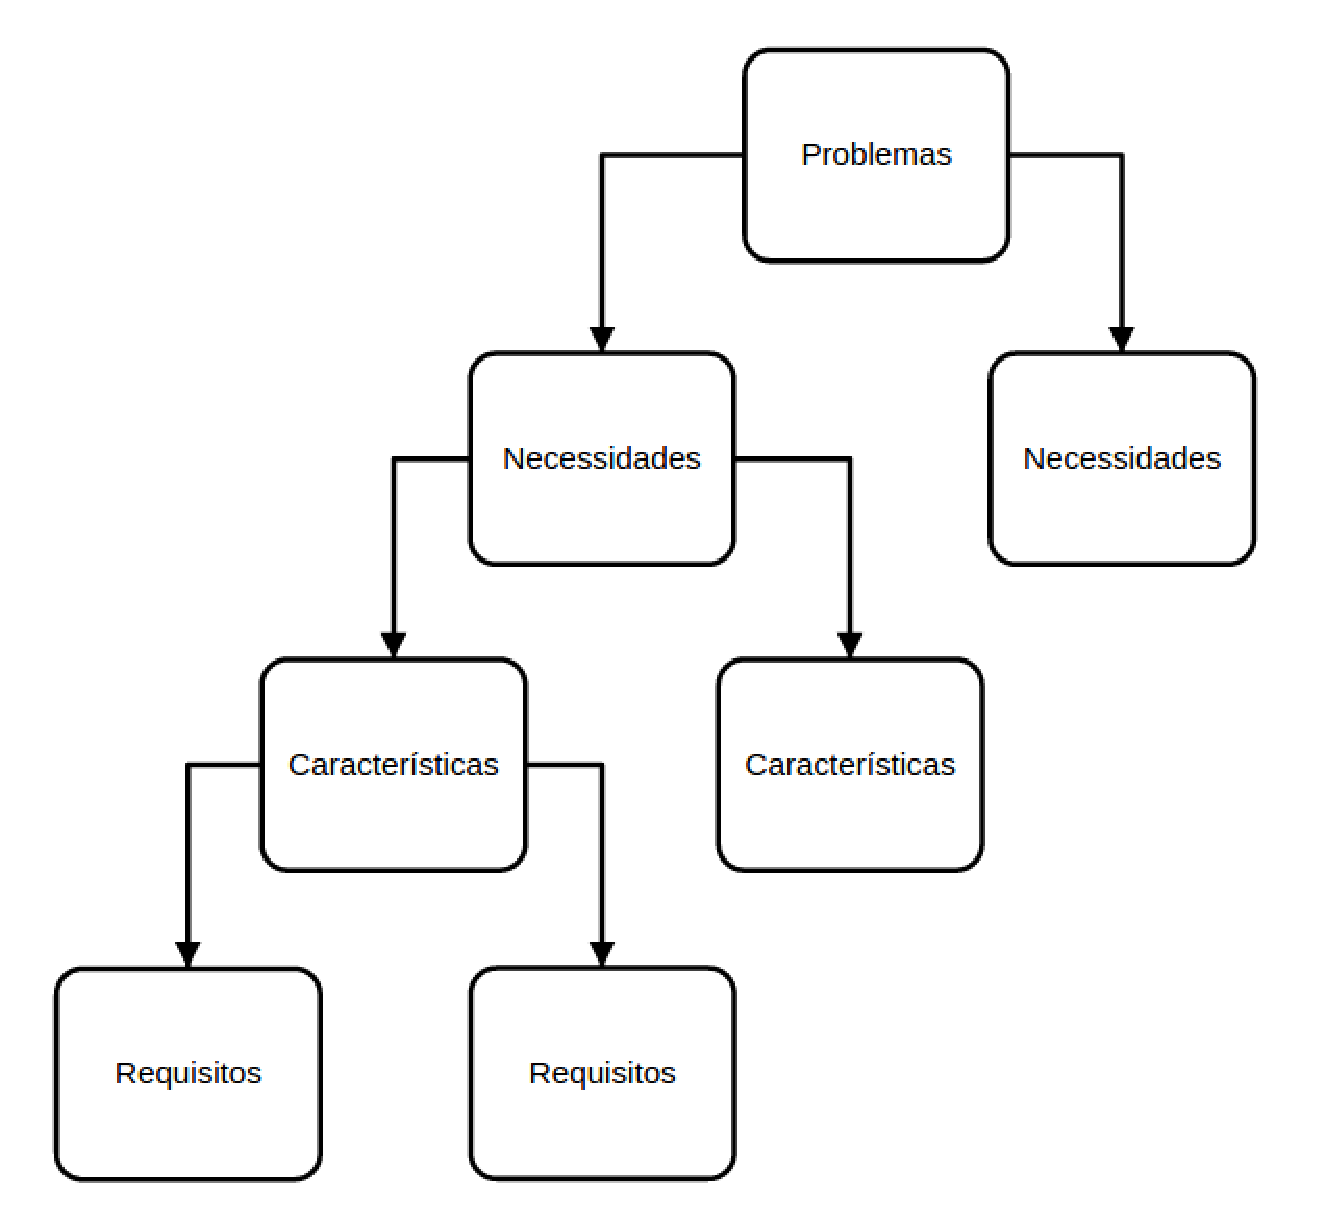
\includegraphics[keepaspectratio=true,scale=0.6]{figuras/rastreabilidade2.eps}
	\caption{Rastreabilidade adotada}
\end{figure}

\clearpage{}

\subsection {Atributos}

De modo geral, todos os nossos itens de rastreabilidade seguem os mesmos atributos, sendo eles

\begin{itemize}

\item{Prioridade;}
\item{Status;}
\item{Dificuldade;}

\end{itemize}

\subsection{Prioridade}

Define o quão importante é o requisito para o sistema em relação aos demais. Os de maior prioridade serão implementados o quanto antes.

\begin{table}[!h]
\centering
\caption{Prioridade}
\label{attr_prioridade}
\begin{tabular}{|p{2cm}|p{8cm}|}
\hline
Alta  & Sinaliza que este requisito é de extrema importância para o sistema e deve ser implementado o quanto antes.                                                            \\ \hline
Média & Sinaliza que este requisito embora importante ele pode ter a sua implementação postergada em favor de um requisito de alta prioridade                                  \\ \hline
Baixa & Um requisito que com a mais baixa prioridade ficará mais para o final do desenvolvimento do sistema ou quando outros requisitos mais importantes já estivem completos. \\ \hline
\end{tabular}
\end{table}

\subsection{Status}

Define o andamento de um determinado requisito durante o desenvolvimento do sistema.

\begin{table}[!h]
\centering
\caption{Status}
\label{attr_Status}
\begin{tabular}{|p{3cm}|p{8cm}|}
\hline
Não inicializado & Usado para sinalizar que o item em questão ainda não foi inicializado, no sentido de que por algum requerimento, como depender de outros itens já terem sido finalizados, este teve o seu desenvolvimento postergado. \\ \hline
Em andamento     & Sinaliza que este item está sendo desenvolvido.                                                                                                                                                                       \\ \hline
Completado       & Sinaliza que este item já foi concluído.                                                                                                                                                                              \\ \hline
\end{tabular}
\end{table}

\subsection{Dificuldade}

Serve de indicativo para uma possível dificuldade na implementação dos requisitos. É um atributo fundamental para o planejamento das iterações.

\begin{table}[!h]
\centering
\caption{Dificuldade}
\label{attr_Dificuldade}
\begin{tabular}{|p{2cm}|p{8cm}|}
\hline
Alta  & Um requisito com um alto este nível de dificuldade receberá uma maior atenção em relação aos demais, pois este pode influenciar fortemente no desenvolvimento do sistema. \\ \hline
Média & Um requisito com este nível não representa um grande risco para a implementação dos sistema.                                                                              \\ \hline
Baixa & Sinaliza que este requisito pode ser facilmente implementado sem maiores riscos ou agravantes.                                                                            \\ \hline
\end{tabular}
\end{table}

\section{Gerenciamento de Mudança de Requisitos}

\subsection{Processamento e Aprovação de Solicitações de Mudança}

De acordo com o nosso processo de software, as aprovações e mudanças serão sempre feitas em concordância com os stakeholders e em etapas bem definidas do processo.

\subsection{Comitê de Controle de Mudança (CCB)}

Havendo uma concordância entre um representante dos stakeholders e os membros do grupo de desenvolvimento, já é considerado como uma mudança válida

\section{Fluxos de Trabalho e Atividades}

Embora qualquer membro do grupo de desenvolvimento do projeto possa estar trabalhando em um determinado requisito, sempre haverá um membro responsável por este, para garantir a completude do mesmo

\section{Treinamento e Recursos}

O próprio grupo de desenvolvimento irá realizar workshops junto aos stakeholders para a realização dos treinamento sobre o uso do sistema.





































\chapter{Especificação Suplementar}
\label{especificação_suplementar}

\section{Introdução}

Este documento tem por finalidade capturar os requisitos de sistema que não foram identificados imediatamente na documentação de requisitos de software do EnGerir. Entre os requisitos não funcionais estão inclusos os atributos de qualidade a serem desenvolvidos, englobando Disponibilidade, Integridade e Segurança e Usabilidade.

\subsection{Finalidade}

Definir os requisitos não funcionais do sistema, sendo estes os que não foram identificados no modelo de casos de uso. Com base na especificação suplementar e no modelo de casos de uso, obtemos todo o conjunto de requisitos do sistema.

\subsection{Escopo}

Prover a gestão dos funcionários da empresa júnior Engrena.

\subsection{Referências}

\begin{itemize}
\item{Artefato - Especificação de Requisitos de Software - Engrena}
\item{Artefato - Especificação de Caso de Uso - Engrena}
\end{itemize}

\section{Funcionalidade}

Os requisitos funcionais estão descritos na especificação de requisitos de software

\section{Usabilidade}

O sistema deverá dispor de uma facilidade em sua utilização, para não ocorrer perca de produtividade para compreender o funcionamento do sistema

\section{Confiabilidade}

O sistema deverá estar disponível 24 horas por dia, 7 dias por semana

\section{Integridade e Segurança}

\begin{itemize}
\item{As informações apresentadas pelo EnGerir deverão estar condizentes impecavelmente baseados na realidade, por demonstrar resultados referentes a funcionários.}
\item{O EnGir deverá ser seguro contra eventualidades, por tratar da produtividade de uma empresa.}
\end{itemize}

\section{Restrição Tecnológica}

\begin{itemize}
\item{A solução web foi proposta para não ocorrer incompatibilidade do sistema, além do fato de que o desempenho de sistemas web é maior.}
\item{A escolha da linguagem de programação, foi a Ruby on Rails, pois ela é a mais eminente dentre a comunidade da FGA, além de ser voltada para o desenvolvimento web.}
\end{itemize}

\section{Restrições de Design}

Por se tratar de uma aplicação web com desenvolvimento em uma linguagem orientada à objetos, o padrão Model-View-Controller (MVC) será utilizado. Esse padrão arquitetural consiste em dividir o sistema em três camadas, consistindo de:

\begin{itemize}
\item{Model: Abstrações das entidades do mundo real no contexto de desenvolvimento. Basicamente, é um modelo lógico do tipo de dado que será armazenado no banco de dados da aplicação}
\item{View: Camada visual do sistema, apresentando as telas para o usuário final para permitir uma interação mais simplificada}
\item{Controller: É a camada que contém a lógica de negócio, com métodos destinados a realizar as funcionalidades prometidas por um determinado software}
\end{itemize}

\begin{figure}[htb]
	\centering
	\label{figura_mvc}
		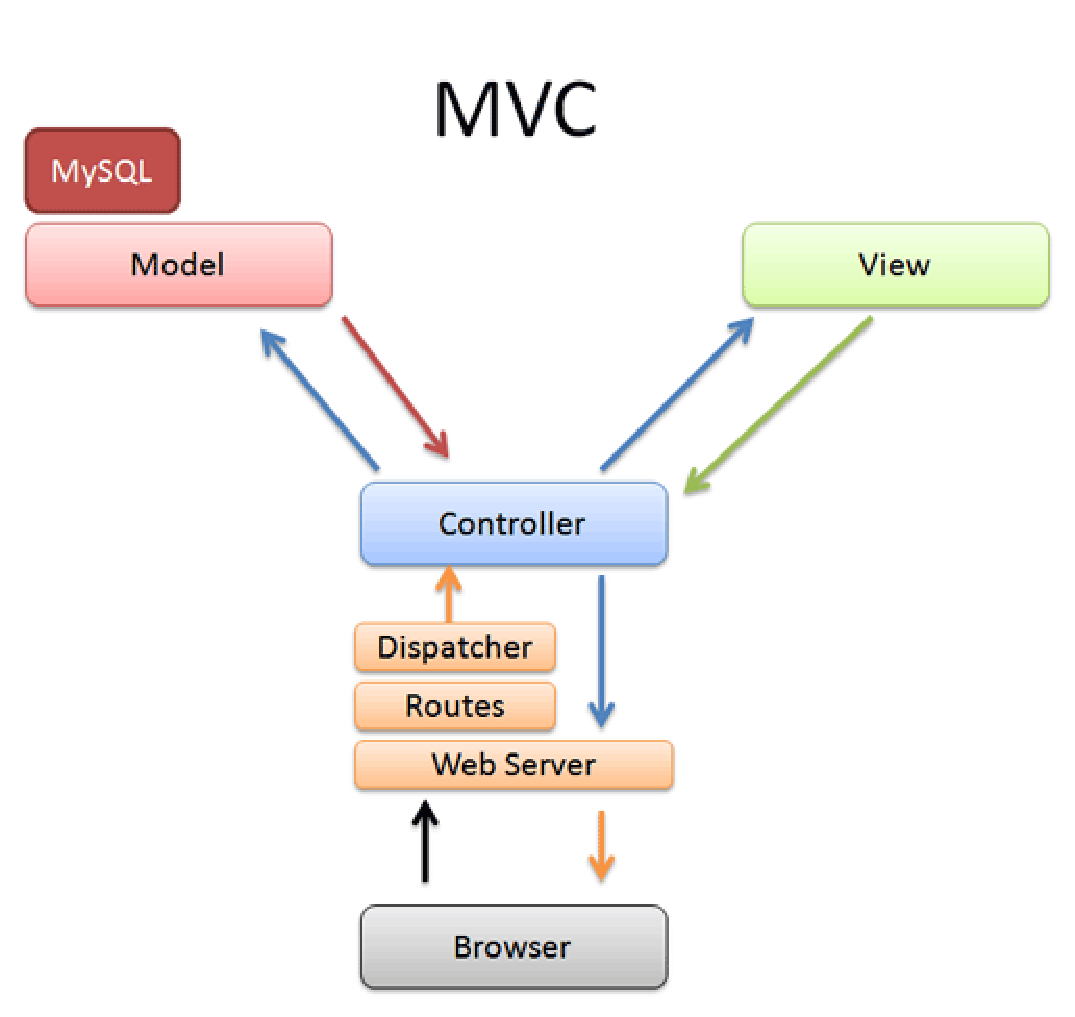
\includegraphics[keepaspectratio=true,scale=0.6]{figuras/MVC.eps}
	\caption{Padrão MVC. Fonte: http://i.stack.imgur.com/Beh3a.png}
\end{figure}

\clearpage{}

\section{Interfaces}

\subsection{Interfaces de Usuário}

\begin{itemize}
  \item{Tela inicial;}
  \item{Tela de administradores;}
  \item{Tela de desempenho;}
  \item{Tela da área da empresa;}
  \item{Tela das tarefas;}
  \item{Tela do diretor;}
  \item{Tela do funcionários.}
\end{itemize}


\subsection{Interfaces de Hardware}

\begin{itemize}
  \item{Servidor para aplicação web;}
  \item{Smartphone;}
  \item{Tablet;}
  \item{Monitor de vídeo;}
  \item{Teclado;}
  \item{Mouse ou touchpad/trackpad.}
\end{itemize}


\subsection{Interfaces de Software}

\begin{itemize}
  \item{Rational Unified Process;}
  \item{Ruby on Rails.}
\end{itemize}

\subsection{Requisitos de Licenciamento}

\begin{itemize}
  \item{A licença atribuída ao sistema será a GPL versão 3}
\end{itemize}




































\chapter{Especificação de Requisitos de Software}
\label{especificação_de_requisitos_de_software}


\section{Introdução}

\subsection{Finalidade}

  Este documento tem por objetivo definir formalmente os requisitos funcionais da aplicação EnGerir, atuando como um contrato com o cliente de que o sistema foi abstraído corretamente pela equipe de desenvolvimento.

  É importante salientar que o comportamento inteiro da aplicação será descrito no documento através dos requisitos funcionais, já que não se trata do desenvolvimento de um subsistema que será acoplado em um sistema maior.

  Os requisitos não funcionais, no entanto, não estarão presentes a seguir. Esses estão descritos na Especificação Suplementar, de forma que a divisão entre o que o sistema deve fazer e como ele deve fazer ficou bem definida.

\subsection{Escopo}

O escopo da aplicação é o de gerenciamento de pessoas de uma empresa júnior. As funcionalidades presentes no mesmo deverão atender às necessidades de tal contexto. É necessário, portanto, mecanismos de gerenciamento de atividades e produtividade.

\subsection{Visão Geral}

Essa Especificação de Requisitos de Software segue a seguinte estrutura de capítulos:

\begin{itemize}
\item{Introdução: tópico ao qual está inserido informações gerais acerca do documento.}
\item{Descrição Geral: uma rápida reflexão acerca do sistema.}
\item{Requisitos Específicos: parte principal do documento que tratará dos requisitos funcionais.}
\item{Classificação dos Requisitos: definição dos atributos aos requisitos funcionais definidos anteriormente.}
\item{Informações de suporte}
\end{itemize}

\section{Descrição Geral}

  As empresas juniores tem o objetivo de preparar os alunos para o mercado de trabalho, prestando os serviços de seus respectivos cursos à um custo mais acessível que grandes corporações da área.

  Por se tratar de um escopo menor, a atuação se dá com um orçamento limitado. Dentro dessa condição financeira, aspectos como produtividade e projetos corretamente elaborados recebem um enorme foco.

  É nesse contexto que entra uma aplicação que permita aos diretores de uma empresa júnior aferir a produtividade de membros e de áreas dentro da empresa, evidenciando áreas que podem precisar de ajustes estruturais para produzirem melhor.

  Indo mais além, o sistema permite aos funcionários terem uma visualização clara de suas atividades e datas de encerramentos, possibilitando um melhor planejamento por parte dos mesmos para o melhor cumprimento de prazos.

\section{Requisitos Específicos}

\subsection{Funcionalidade}

  Nesta seção, serão descritos os requisitos funcionais obtidos através da utilização das técnicas de elicitação citadas no primeiro relatório da disciplina. Como descrito no mesmo, os requisitos serão avaliados com base em três atributos:

\begin{itemize}
\item{
  Prioridade

  \begin{itemize}
    \item{Alta}
    \item{Média}
    \item{Baixa}
  \end{itemize}
}
\item{
  Status

  \begin{itemize}
    \item{Completado}
    \item{Em andamento}
    \item{Não inicializado}
  \end{itemize}
}
\item{
  Dificuldade

  \begin{itemize}
    \item{Alta}
    \item{Média}
    \item{Baixa}
  \end{itemize}
}
\end{itemize}

Desses atributos, apenas prioridade e dificuldade serão descritos nesse documento, enquanto que status será utilizado para rastreabilidade no desenvolvimento da aplicação.


\subsection{RF 1.1.1.1  Anexar documento à tarefas}

\begin{itemize}
  \item{Prioridade: Média}
  \item{Dificuldade: Alta}
  \item{Status: Não inicializado}
\end{itemize}

Deve ser possível anexar documentos à tarefas criadas com o objetivo de fornecer mais informações e detalhes para o funcionário designado sobre o que está sendo pedido dele. Essas informações podem vir na forma de templates, livros ou qualquer outro tipo de documento.


\subsection{RF 1.1.1.2 Buscar por competência}

\begin{itemize}
  \item{Prioridade: Baixa}
  \item{Dificuldade: Alta}
  \item{Status: Não inicializado}
\end{itemize}

O gestor, para alocação de pessoas à um projeto, deve poder buscar por pessoas na aplicação utilizando um filtro de competência, com o objetivo de atribuir o projeto às pessoas mais adequadas ao mesmo.


\subsection{RF 1.1.1.3 Realizar backup}

\begin{itemize}
  \item{Prioridade: Alta}
  \item{Dificuldade: Alta}
  \item{Status: Não inicializado}
\end{itemize}

O sistema deverá realizar backups de forma constante, para que não se percam todos os dados na ocorrência de alguma eventualidade, tanto a nível de software quanto hardware.


\subsection{RF 1.1.1.4 Realizar login com Facebook e Google+}

\begin{itemize}
  \item{Prioridade: Baixa}
  \item{Dificuldade: Média}
  \item{Status: Não inicializado}
\end{itemize}

O sistema deve permitir o login através de uma conta do Facebook ou do Google+ para facilitar o acesso a ferramenta.


\subsection{RF 1.1.1.5 Cadastrar membros}

\begin{itemize}
  \item{Prioridade: Alta}
  \item{Dificuldade: Baixa}
  \item{Status: Em andamento}
\end{itemize}

O sistema deve ser capaz de cadastrar novos membros.


\subsection{RF 1.1.1.6 Remover membros}

\begin{itemize}
  \item{Prioridade: Alta}
  \item{Dificuldade: Baixa}
  \item{Status: Em andamento}
\end{itemize}

O sistema deve ser capaz de remover logicamente os membros.


\subsection{RF 1.1.1.7 Atualizar membros}

\begin{itemize}
  \item{Prioridade: Alta}
  \item{Dificuldade: Baixa}
  \item{Status: Em andamento}
\end{itemize}

O sistema deve ser capaz de atualizar os dados de seus membros.



\subsection{RF 1.1.1.8 Visualizar membros}

\begin{itemize}
  \item{Prioridade: Baixa}
  \item{Dificuldade: Baixa}
  \item{Status: Não inicializado}
\end{itemize}

O sistema deve ser capaz de disponibilizar a visualização dos dados de seus membros.


\subsection{RF 1.1.2.1 Inserir competências e áreas}

\begin{itemize}
  \item{Prioridade: Baixa}
  \item{Dificuldade: Baixa}
  \item{Status: Não inicializado}
\end{itemize}

Na criação do usuário e na edição do mesmo, o funcionário deve poder inserir suas competências técnicas em sua descrição e as áreas da empresa para qual o mesmo já trabalhou, de forma a manter os gestores cientes da rotatividade realizada pelo usuário


\subsection{RF 1.1.2.2 Gerar desempenho por mês}

\begin{itemize}
  \item{Prioridade: Alta}
  \item{Dificuldade: Média}
  \item{Status: Em andamento}
\end{itemize}

Além de visualizar graficamente o desempenho de uma área ou de um membro, deve ser possível separar essa informação por meses. Isso é, o sistema deve permitir a visualização da produtividade de um funcionário ou de uma área em um determinado mês, para fins de comparação com outros períodos de tempo.


\subsection{RF 1.2.1.1 Criar Tarefas}

\begin{itemize}
  \item{Prioridade: Alta}
  \item{Dificuldade: Baixa}
  \item{Status: Em andamento}
\end{itemize}

O sistema deve disponibilizar o cadastro de tarefas para os seus membros.


\subsection{RF 1.2.1.2 Remover Tarefas}

\begin{itemize}
  \item{Prioridade: Alta}
  \item{Dificuldade: Baixa}
  \item{Status: Em andamento}
\end{itemize}

O sistema deve excluir logicamente as tarefas.


\subsection{RF 1.2.1.3 Atualizar Tarefas}

\begin{itemize}
  \item{Prioridade: Alta}
  \item{Dificuldade: Baixa}
  \item{Status: Em andamento}
\end{itemize}

O sistema deve disponibilizar formas de manter as tarefas atualizadas.


\subsection{RF 1.2.1.4 Visualizar Tarefas}

\begin{itemize}
  \item{Prioridade: Alta}
  \item{Dificuldade: Baixa}
  \item{Status: Em andamento}
\end{itemize}

O sistema deve disponibilizar formas dos membros poderem visualizar as suas tarefas.


\subsection{RF 1.2.1.5 Gerar Notificação para Membros Quando uma Tarefa for Criada}

\begin{itemize}
  \item{Prioridade: Média}
  \item{Dificuldade: Média}
  \item{Status: Não inicializado}
\end{itemize}

Ao atribuir uma tarefa para um funcionário, o mesmo deve receber uma notificação para ser informado da existência da tarefa.


\subsection{RF 1.2.1.6 Atribuir Tarefa a Funcionários}

\begin{itemize}
  \item{Prioridade: Alta}
  \item{Dificuldade: Baixa}
  \item{Status: Em andamento}
\end{itemize}

Após a criação de uma tarefa, o gestor da empresa deve poder atribuí-la à um funcionário da mesma.


\subsection{RF 1.2.2.1 Atribuir Notas às Tarefas}

\begin{itemize}
  \item{Prioridade: Baixa}
  \item{Dificuldade: Baixa}
  \item{Status: Não inicializado}
\end{itemize}

O gestor de uma área pode atribuir uma nota a uma tarefa enviada por um funcionário, de forma a servir como parâmetro no futuro para decisões como promoção de um membro à um cargo de diretoria e outras decisões.


\subsection{RF 1.2.2.2 Gerar Notificação para os Diretores Quando um Membro Finalizar}

\begin{itemize}
  \item{Prioridade: Média}
  \item{Dificuldade: Média}
  \item{Status: Não inicializado}
\end{itemize}

Após um funcionário assinalar uma tarefa como completa, uma notificação deve ser gerada para o gestor daquela área com o objetivo de conscientizar o mesmo desse fato, para que ele possa recolher pessoalmente a atividade com o membro.


\subsection{RF 1.2.3.1 Cadastrar Área}

\begin{itemize}
  \item{Prioridade: Alta}
  \item{Dificuldade: Baixa}
  \item{Status: Em andamento}
\end{itemize}

O sistema deve disponibilizar o cadastro de áreas para os seus membros, cada membro pertence a uma área.


\subsection{RF 1.2.3.2 Remover Área}

\begin{itemize}
  \item{Prioridade: Alta}
  \item{Dificuldade: Baixa}
  \item{Status: Em andamento}
\end{itemize}

O sistema deve disponibilizar a remoção lógica de suas áreas.


\subsection{RF 1.2.3.3 Atualizar Área}

\begin{itemize}
  \item{Prioridade: Alta}
  \item{Dificuldade: Baixa}
  \item{Status: Em andamento}
\end{itemize}

O sistema deve possibilitar manter as áreas atualizadas.


\subsection{RF 1.2.3.4 Visualizar Área}

\begin{itemize}
  \item{Prioridade: Alta}
  \item{Dificuldade: Baixa}
  \item{Status: Em andamento}
\end{itemize}

O sistema deve possibilitar a visualização de suas áreas.



\section{Restrições de Design}

Neste tópico, serão apresentados as restrições para o projeto da ferramente, que se concentram em uma restrição de linguagem e de framework, além das ferramentas que auxiliam o desenvolvimento.

\subsection{Ruby on Rails}

Por se tratar do desenvolvimento de uma ferramenta web, uma das melhores linguagens disponíveis para esse projeto é o Ruby, capaz de formar um código altamente legível e de fácil manutenção no futuro.

Para complementar, será utilizado o framework Rails, que direciona a linguagem para o desenvolvimento web, com diversos recursos para facilitar a criação de objetos e entidades no projeto orientado à objeto.

\subsection{Git}

Ferramenta de versionamento que será utilizada no desenvolvimento do projeto, para manter controle dos arquivos e alterações da ferramenta.


\subsection{Innoslate}

Ferramenta de gerenciamento de requisitos que será utilizada para realizar a rastreabilidade vertical do projeto.

Sobre a ferramenta, é importante ressaltar que é uma ferramenta paga que será utilizada no período trial.

\section{Requisitos de Licenciamento}

O software EnGerir tem o objetivo de ser gratuito e de livre distribuição para qualquer pessoa ou empresa que tenha o objetivo de utilizá-lo ou desenvolver outro software com base no código do mesmo.

Isso significa que, à qualquer momento, o projeto pode ser utilizado para qualquer fim por terceiros. Qualquer empresa que tiver as dificuldades encontradas pela Engrena poderá utilizar a solução entregue à mesma.

A licença, portanto, será a General Public License V3 (GPL), amplamente utilizada no contexto de software livre, que é precisamente onde o EnGerir se encaixa.






























\chapter{Diagrama de Casos de Uso}
\label{use-diagram}


\begin{figure}[htb]
	\centering
	\label{figura_Diagrama-de-Caso-de-Uso}
		\includegraphics[keepaspectratio=true,scale=0.6]{figuras/Diagrama-de-Caso-de-Uso.eps}
	\caption{Diagrama de Caso de Uso}
\end{figure}

\clearpage{}



\chapter{Especificação de Caso de Uso}
\label{especificação_de_caso_de_uso}


\section{UC01 - Manter Membro}

\subsection{Descrição}

Esse caso de uso é destinado aos futuros funcionários da Engrena, que desejam obter um cadastro na aplicação. Também é utilizado pelos gestores da empresa, pois podem remover membros inativos e/ou expulsos.

\subsection{Atores}

\begin{itemize}
  \item{Gestores da Engrena}
  \item{Funcionário da Engrena}
\end{itemize}

\subsection{Fluxo de Eventos}

\textbf{Fluxo Principal}
\begin{enumerate}
  \item{O Usuário preenche o formulário de cadastro} %1
  \item{O Usuário envia o formulário para o sistema} %2
  \item{O sistema valida os dados do usuário [RN01]} %3
  \item{O sistema realiza o cadasto do usuário} %4
\end{enumerate}

\textbf{Fluxo Alternativo}

[FA01] - Excluir um membro
\begin{enumerate}
  \item{O usuário solicita ao sistema a exclusão de um membro}
  \item{O sistema solicita confirmação}
  \item{O usuário confirma a ação}
  \item{O sistema então, desabilita o membro, realizando a exclusão lógica}
  \item{O caso de uso é encerrado}
\end{enumerate}

[FA02] - Editar um membro
\begin{enumerate}
  \item{O usuário decide editar um membro}
  \item{O sistema carregará o formulário de dados}
  \item{O usuário altera as informações nos campos que desejar}
  \item{O usuário solicita ao sistema a alteração dos dados}
  \item{O caso de uso é encerrado}
\end{enumerate}

[FA03] - Mostrar membros
\begin{enumerate}
  \item{O Usuário solicita vi visualização de membros do sistema}
  \item{O sistema lista os membros}
  \item{O caso de uso é encerrado}
\end{enumerate}

\textbf{Fluxo de Exceção}
[FE01] - Cadastro inválido
\begin{enumerate}
\item{Sistema informa ao Usuário os campos inválidos.}
\item{O Usuário preenche os campos inválidos.}
\item{O Usuário envia o formulário para o sistema.}
\item{Retorna para o passo 4 do fluxo principal.}
\end{enumerate}


\subsection{Condições Prévias}
\begin{itemize}
\item{Esse caso de uso é iniciado quando o usuário está no sistema como administrador e deseja cadastrar ou remover uma área que representa uma direção, bem como atualizá-la ou apenas ler sobre a mesma.}
\end{itemize}

\subsection{Condições Posteriores}

Redirecionamento para o perfil da área. Ao final do caso de uso, o usuário deve ser redirecionado para a página da área.


\section{UC02 - Manter Área}

\subsection{Descrição}

Esse caso de uso é destinado aos administradores do sistema, que poderão criar áreas dentro da aplicação que representam as mesmas na empresa.

\subsection{Atores}

\begin{itemize}
  \item{Gestores da Engrena}
\end{itemize}

\subsection{Fluxo de eventos}

\textbf{Fluxo Principal}

Esse caso de uso é iniciado quando o usuário está no sistema como administrador e deseja cadastrar ou remover uma área que representa uma direção, bem como atualizá-la ou apenas ler sobre a mesma

\begin{enumerate}
  \item{O usuário segue para a página de áreas, onde estarão listadas as que já existem com as opções de excluir [FA01], editar [FA02] e mostrar [FA03] a área. O usuário decide cadastrar uma nova área.}
  \item{O usuário preenche os campos do formulário}
  \item{O sistema valida as informações [RN02]}
  \item{O sistema redireciona o usuário para o perfil da área, onde estão presentes as opções}
\end{enumerate}


\textbf{Fluxo Alternativo}

[FA01] - Excluir uma área
\begin{enumerate}
  \item{O usuário solicita a exclusão de uma área}
  \item{Uma mensagem de confirmação aparecerá}
  \item{O usuário confirma a ação}
  \item{O sistema então, desabilita a área, realizando a exclusão lógica}
  \item{O caso de uso é encerrado}
\end{enumerate}


[FA02] - Editar uma área
\begin{enumerate}
  \item{O usuário decide editar uma área}
  \item{O sistema carrega o formulário de dados}
  \item{O usuário altera as informações nos campos que desejar}
  \item{O usuário salva as mudanças por meio de um botão}
  \item{O caso de uso é encerrado}
\end{enumerate}


[FA03] - Mostrar uma área
\begin{enumerate}
  \item{O Usuário solicita a visualização de áreas ao sistema}
  \item{O Usuário seleciona uma área}
  \item{O sistema redireciona para a página da área, que conterá informações gerais sobre a mesma}
  \item{O caso de uso é encerrado}
\end{enumerate}

\subsection{Condições Prévias}

\begin{itemize}
\item{Para realizar todas as funcionalidades previstas nesse caso de uso, o usuário deve estar no sistema como administrador, tendo total acesso à todas as partes da aplicação}
\end{itemize}

\subsection{Condições Posteriores}

Redirecionamento para o perfil da área. Ao final do caso de uso, o usuário deve ser redirecionado para a página da área


\section{UC03 - Manter tarefas}

\subsection{Descrição}

Este caso de uso é predominantemente destinado aos administradores que poderão criar tarefas e concedê-las aos usuários, que por sua vez, poderão visualizá-las.


\subsection{Atores}

\begin{itemize}
  \item{Gestores da Engrena}
  \item{Usuários da aplicação que seriam os funcionários da engrena}
\end{itemize}

\subsection{Fluxo de eventos}

\textbf{Fluxo principal}

\begin{enumerate}
  \item{O usuário segue para a página de tarefas, onde estarão listadas as que já existem com as opções de excluir [FA01], editar [FA02] e mostrar [FA03] a tarefa. O usuário deseja cadastrar uma nova área}
  \item{O usuário preenche os campos do formulário}
  \item{O sistema valida as informações [RN03]}
  \item{O sistema redireciona o usuário para o perfil das tarefas, onde estarão presentes as opções}
\end{enumerate}


\textbf{Fluxo Alternativo}

[FA01] - Excluir uma tarefa
\begin{enumerate}
  \item{O usuário deseja excluir uma tarefa}
  \item{Uma mensagem de confirmação aparece}
  \item{O usuário confirma a ação}
  \item{O sistema então, desabilita a área, realizando a exclusão lógica}
  \item{O caso de uso é encerrado}
\end{enumerate}


[FA02] - Editar uma tarefa
\begin{enumerate}
  \item{O usuário deseja editar uma tarefa}
  \item{O sistema carrega o formulário de dados}
  \item{O usuário altera as informações nos campos que desejar}
  \item{O usuário salva as mudanças por meio de um botão}
  \item{O caso de uso é encerrado}
\end{enumerate}


[FA03] - Mostrar uma tarefa
\begin{enumerate}
  \item{O Usuário solicita ao sistema as suas tarefas}
  \item{O Usuário seleciona uma de suas tarefas}
  \item{O sistema redireciona o Usuário para a página com as informações da tarefa}
  \item{O caso de uso é encerrado}
\end{enumerate}

\subsection{Condições Prévias}
\begin{itemize}
\item{Para realizar todas as funcionalidades previstas nesse caso de uso, o usuário deve estar no sistema como administrador, tendo total acesso à todas as partes da aplicação. Ou deve estar no sistema como usuário, tendo acesso apenas a visualização das suas tarefas}
\end{itemize}

\subsection{Condições Posteriores}

Redirecionamento para o perfil da tarefa. Ao final do caso de uso, o usuário, administrador ou usuário deve ser redirecionado para a página da tarefa.


\section{UC04 - Atribuir tarefas à funcionário}

\subsection{Descrição}

Esse caso de uso é destinado gestores da Engrena, que poderão assinalar responsáveis para tarefas.

\subsection{Atores}

\begin{itemize}
  \item{Gestores da Engrena}
\end{itemize}


\subsection{Fluxo de Eventos}

\textbf{Fluxo Principal}

\begin{enumerate}
  \item{O Usuário segue para a parte de tarefas do sistema}
  \item{O Usuário clica no nome de uma tarefa}
  \item{O sistema redireciona para a página daquela tarefa}
  \item{O Usuário clica no campo que indica o responsável pela tarefa}
  \item{O Usuário preenche o novo responsável pela tarefa}
  \item{O sistema valida a informação [RN04]}
  \item{Uma mensagem de confirmação aparece}
  \item{O Usuário confirma a ação}
  \item{O caso de uso é encerrado}
\end{enumerate}

\subsection{Condições Prévias}
\begin{itemize}
\item{Para realizar todas as funcionalidades previstas nesse caso de uso, o usuário deve estar logado no sistema como administrador}
\end{itemize}

\subsection{Condições Posteriores}

Redirecionamento para o perfil da tarefa. Ao final do caso de uso, o usuário deve ser redirecionado para a página da tarefa.


\section{UC05 - Gerar gráficos de produtividade de membros e área}

\subsection{Descrição}

Esse caso de uso é destinado ao gestor da Engrena que deseja visualizar o desempenho de um membro ou alguma área para ser capaz de tomar as melhores decisões estratégicas possíveis.

\subsection{Atores}

\begin{itemize}
  \item{Gestores da Engrena}
\end{itemize}


\subsection{Fluxo de Eventos}


\textbf{Fluxo Principal}

\begin{enumerate}
  \item{O usuário entra na página de um membro ou área}
  \item{O sistema apresenta um gráfico que representará a produtividade da área}
  \item{O caso de uso encerrado}
\end{enumerate}

\subsection{Condições Prévias}
\begin{itemize}
\item{Para realizar todas as funcionalidades previstas nesse caso de uso, o usuário deve estar logado no sistema com sua conta de usuário comum.}
\end{itemize}



\section{UC06 - Assinalar status das tarefas}

\subsection{Descrição}

Esse caso de uso é destinado aos funcionários da Engrena, que poderão assinalar a porcentagem de conclusão de uma tarefa

\subsection{Atores}

\begin{itemize}
  \item{Funcionários da Engrena}
\end{itemize}

\subsection{Fluxo de Eventos}

\textbf{Fluxo Principal}

\begin{enumerate}
  \item{O usuário segue para a sua área de tarefas, onde estarão todas que foram atribuídas ao mesmo}
  \item{O Usuário clica no nome de uma tarefa}
  \item{O sistema redireciona para a página daquela tarefa}
  \item{O Usuário atualiza o campo de status na página principal}
  \item{O sistema valida a entrada do usuário [RN05]}
  \item{Uma mensagem de confirmação aparece}
  \item{O Usuário confirma a ação}
  \item{O caso de uso é encerrado}
\end{enumerate}

\subsection{Condições Prévias}
\begin{itemize}
\item{Para realizar todas as funcionalidades previstas nesse caso de uso, o usuário deve estar logado no sistema com sua conta de usuário comum}
\end{itemize}

\subsection{Condições Posteriores}

Redirecionamento para o perfil da tarefa. Ao final do caso de uso, o usuário deve ser redirecionado para a página da tarefa



\section{Regras de Negócio}

\subsection{[RN01] - Validação de Informações}

\begin{table}[!h]
\centering
\caption{RN01}
\label{RN01}
\begin{tabular}{|p{4cm}|p{8cm}|p{3cm}|}
\hline
Nome do campo                     & Formato                             & Obrigatoriedade \\ \hline
Nome do membro                    & Texto com, no máximo, 50 caracteres & Sim             \\ \hline
Descrição                         & Texto, sem limitação de caracteres  & Sim             \\ \hline
Áreas da empresa em que trabalhou & Texto, sem limitação de caracteres  & Opcional        \\ \hline
\end{tabular}
\end{table}

\clearpage{}


\subsection{[RN02] - Validação de Informações}

\begin{table}[!h]
\centering
\caption{RN02}
\label{RN02}
\begin{tabular}{|p{4cm}|p{8cm}|p{3cm}|}
\hline
Nome do campo   & Formato                             & Obrigatoriedade \\ \hline
Nome da área    & Texto com, no máximo, 40 caracteres & Sim             \\ \hline
Descrição       & Texto, sem limitação de caracteres  & Sim             \\ \hline
Nome do diretor & Texto com, no máximo, 30 caracteres & Não             \\ \hline
\end{tabular}
\end{table}


\subsection{[RN03] - Validação de Informações}

\begin{table}[!h]
\centering
\caption{RN03}
\label{RN03}
\begin{tabular}{|p{4cm}|p{8cm}|p{3cm}|}
\hline
Nome do campo          & Formato                             & Obrigatoriedade \\ \hline
Nome da área           & Texto com, no máximo, 40 caracteres & Sim             \\ \hline
Descrição              & Texto, sem limitação de caracteres  & Sim             \\ \hline
Nome do diretor        & Texto com, no máximo, 30 caracteres & Não             \\ \hline
Destinatário da Tarefa & Texto com, no máximo, 40 caracteres & Não             \\ \hline
\end{tabular}
\end{table}


\subsection{[RN04] - Validação de Informações}

\begin{table}[!h]
\centering
\caption{RN04}
\label{RN04}
\begin{tabular}{|p{4cm}|p{8cm}|p{3cm}|}
\hline
Nome do campo          & Formato                             & Obrigatoriedade \\ \hline
Nome do responsável    & Texto com, no máximo, 20 caracteres & Sim             \\ \hline
\end{tabular}
\end{table}


\subsection{[RN05] - Validação de Informações}

\begin{table}[!h]
\centering
\caption{RN05}
\label{RN05}
\begin{tabular}{|p{4cm}|p{8cm}|p{3cm}|}
\hline
Nome do campo          & Formato                                                    & Obrigatoriedade \\ \hline
Status da tarefa       & Dropdown com as seguintes porcentagens: 0, 25, 50, 75, 100 & Sim             \\ \hline
\end{tabular}
\end{table}












\chapter{Plano de Iteração}
\label{iteration}


\section{Introdução}
Este plano de iteração irá detalhar em ordem cronológica as iterações e suas respectivas atividades executadas ao longo de todo o projeto.

\subsection{Finalidade}
Tem como finalidade explicar e detalhar como será realizada a implementação do EnGerir, esclarecendo tudo que será executado e quando será executado, para todas as partes envolvidas.

\subsection{Escopo}
O plano de iteração do projeto EnGerir foca no detalhamento das atividades executadas durante a etapa de construção do \textit{software}.

\subsection{Definições, Acrônimos e Abreviações}
\begin{itemize}
\item \textit{Template}: modelo estabelecido a fim de criar conteúdos de forma otimizada.
\end{itemize}

\subsection{Visão Geral}
\begin{itemize}
\item As principais atividades de cada iteração;
\item Os recursos humanos necessários;
\item Os casos de uso priorizados para cada iteração;
\item Os critérios de avaliação de cada iteração.
\end{itemize}

\subsection{Referências}
Este plano de iteração foi escrito seguindo o \textit{template} disponibilizado no seguinte endereço eletrônico: www.funpar.ufpr.br

\section{Plano}

\begin{table}[!h]
\centering
\caption{Plano de iteração}
\label{iteration-plan}
\begin{tabular}{|l|l|l|}
\hline
Atividade                                  & Início   & Termínio \\ \hline
Atualização do cronograma                  & 04/06/16 & 20/06/16 \\ \hline
Priorizar casos de uso                     & 14/06/16 & 14/06/16 \\ \hline
Definir casos de uso atacados por iteração & 10/06/16 & 14/06/16 \\ \hline
Primeira Iteração                          & 12/06/16 & 20/06/16 \\ \hline
\end{tabular}
\end{table}

\clearpage{}

\section{Recursos}
A equipe de trabalho consiste de quatro integrantes:
\begin{itemize}
\item Fábio Teixeira
\item Gustavo Araujo
\item Marcelo Martins
\item Victor Navarro
\end{itemize}

\section{Casos de Uso}
Para a 1ª iteração, serão implementados os seguintes casos de uso:
\begin{itemize}
\item UC01- Manter membros;
\item UC02- Manter área;
\item UC03- Manter tarefas;
\item UC04- Atribuir tarefas à funcionário;
\item UC05- Gerar gráficos de produtividade de membros e área;
\item UC06- Assinalar \textit{status} das tarefas.
\end{itemize}

\section{Critérios de Avaliação}
\begin{itemize}
\item Cumprimento dos prazos;
\item Implementação dos casos de uso.
\end{itemize}















\end{apendicesenv}
